\chapter[SAX-P]{Symbolic representation of cyclic time series based on properties of cycles}
\begin{abstract} 
The analysis of cyclic time series from bio-mechanics is based on the
comparison of the properties of their cycles. As usual algorithms of time 
series classification ignore this particularity, we propose
a symbolic representation of cyclic time series based on the properties
of cycles, named SAX-P. The resulting character strings can be compared
using the Dynamic Time Warping distance. The application of SAX-P
to propulsive moments of three subjects (S1, S2, S3) moving in Manual
Wheelchair highlight the asymmetry of their propulsion. The symbolic representation 
SAX-P facilitates the reading of
the cyclic time series and the clinical interpretation of the classification results.

\end{abstract} 

\section{Introduction}
\label{introduction}

Generally, during his locomotion, the human being performs cyclic movements (eg walking, running, swimming,
cycling). The bio-mechanical analysis of these movements is performed with various measuring instruments 
(eg force and acceleration sensors, kinematic analysis systems) that enable continuous recording over 
long periods of many kinematic and dynamic parameters. These recordings produce long
time series composed of many cycles or patterns, representative of the movements made and effort 
produced by the subject during his displacement (Fig. \ref{fig:cyclicTS}).


 \begin{figure}[h]
  \centering
   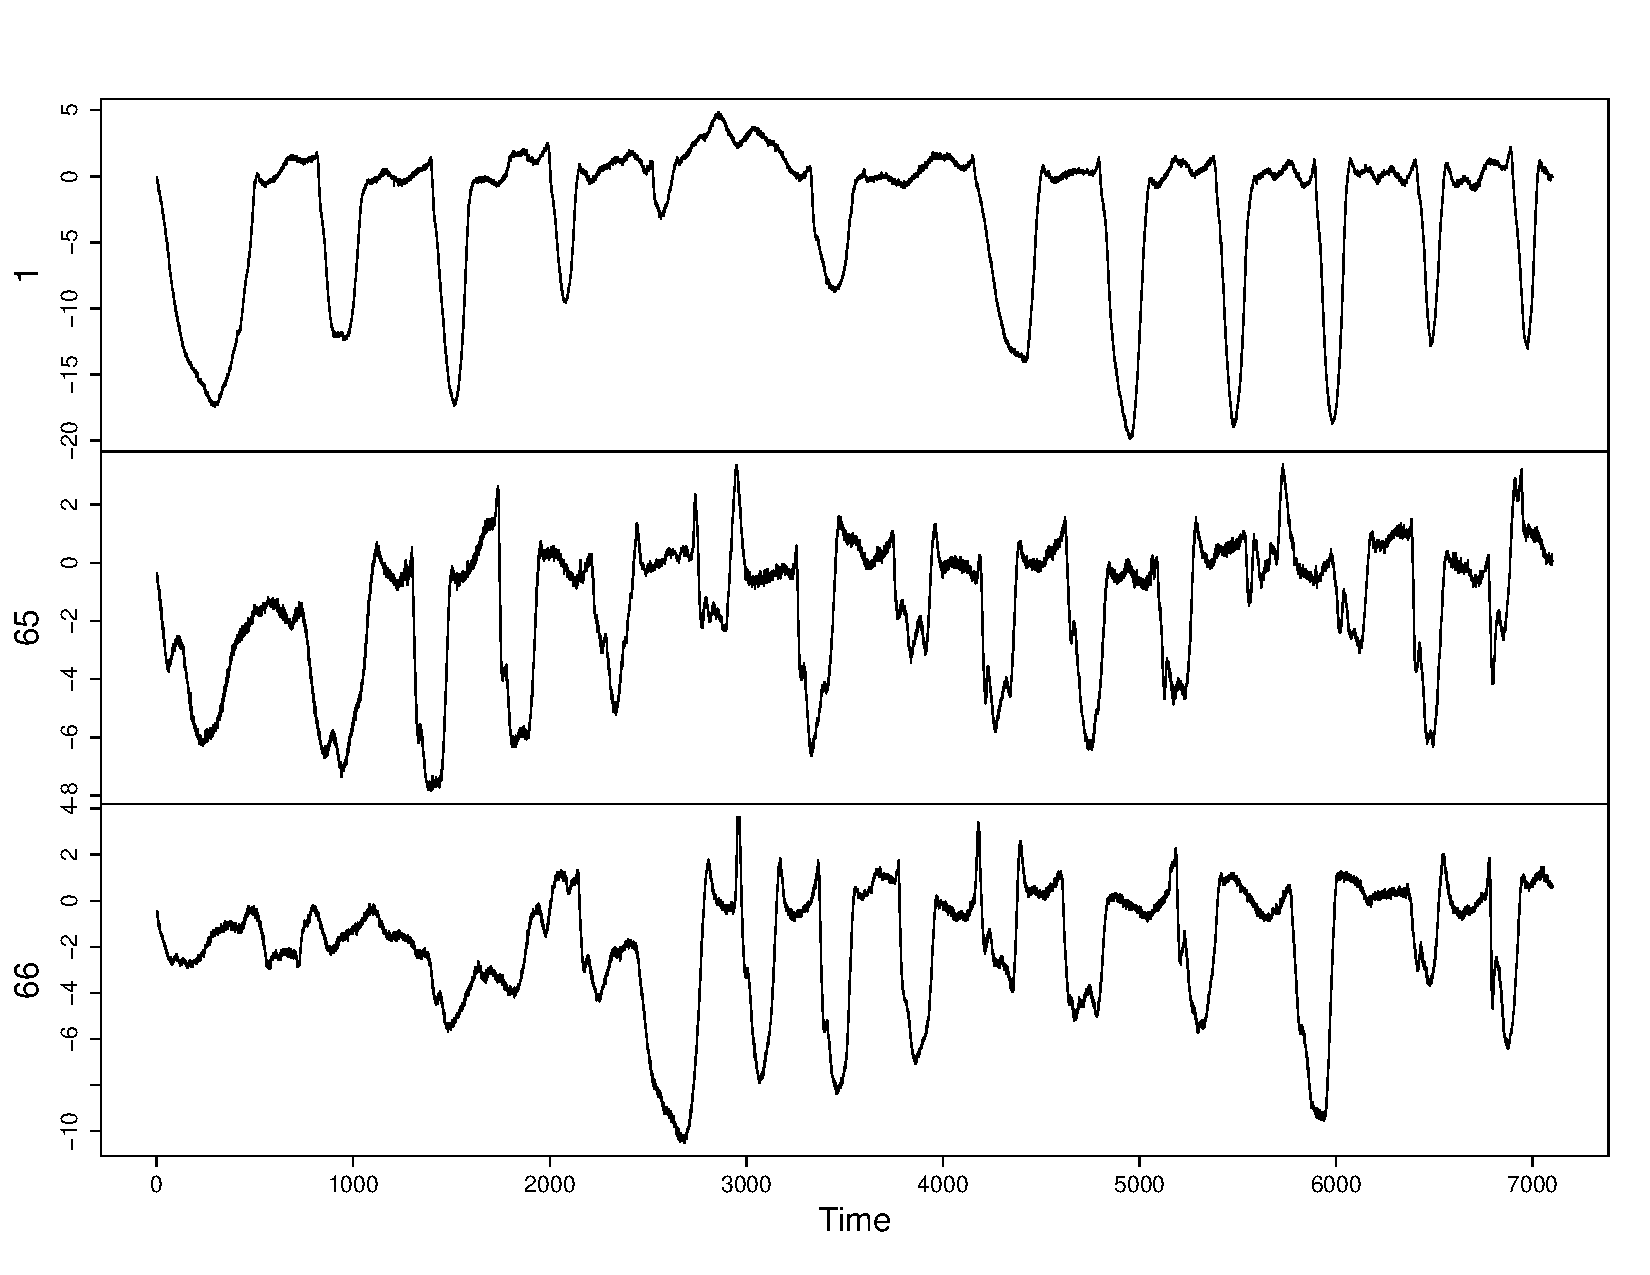
\includegraphics[scale=0.4]{images/sax-p/cycliqueTS}
    \caption{Cyclic time series form manual wheelchair locomotion}
  \label{fig:cyclicTS}
  \end{figure}


These cycles are the time series analysis units and have several
characteristic properties such as the minimum value, the area under the cycle 
\cite{Vegter2014} (Fig. \ref{fig:cycleProp}). 

 \begin{figure}[h]
  \centering
   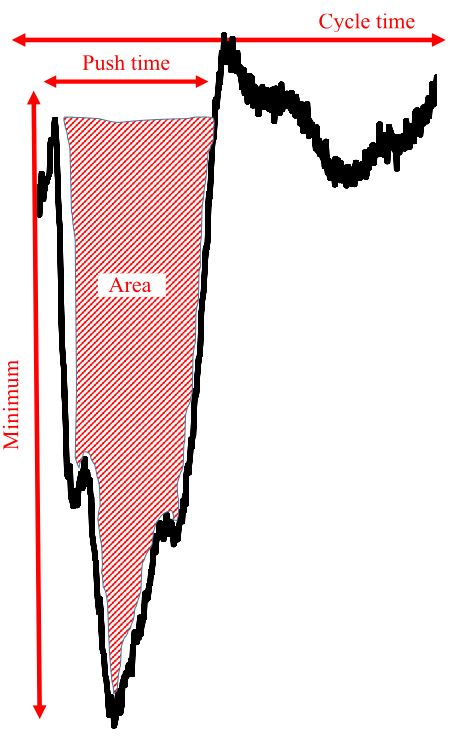
\includegraphics[scale=0.4]{images/sax-p/cycle_prop}
    \caption{Properties of a cycle}
  \label{fig:cycleProp}
  \end{figure}
	

For comparing time series, several previous studies suggested to break them into 
small segments and then to compare the properties of their segments.
A segment of a time series is a sequence of consecutive values belonging to it \cite{Abonyi2003}.


\cite{keogh2001dimensionality} proposed replacing each segment of a time series
$X=x_{1},x_{2},\cdots,x_{n}$ by its mean values;
$\bar{x}_{i}=\frac{N}{n}\sum_{j=\frac{n}{N}(i-1)+1}^{(\frac{n}{N})i}x_{j}$  transforming the time
series, which is a sequence of values, in the suite of the means of its N segments
$\bar{X}=\bar{x}_{1}\bar{,x}_{2},\cdots,\bar{x}_{N}$ This method is known as Piecewise Aggregate
Approximation (PAA) (Fig. \ref{fig:paa}). The time series $C$ and $Q$ are then compared by calculating the distance $DR$
between the suite $\bar{C}$ and $\bar{Q}$ of the means of their segments :
\begin{equation}
DR(\bar{C},\bar{Q})=\sqrt{\frac{n}{N}\sum_{i=1}^{N}(\bar{c}_{i}-\bar{q}_{i})^{2}}
\label{equ:paa}
\end{equation}

 \begin{figure}[h]
  \centering
   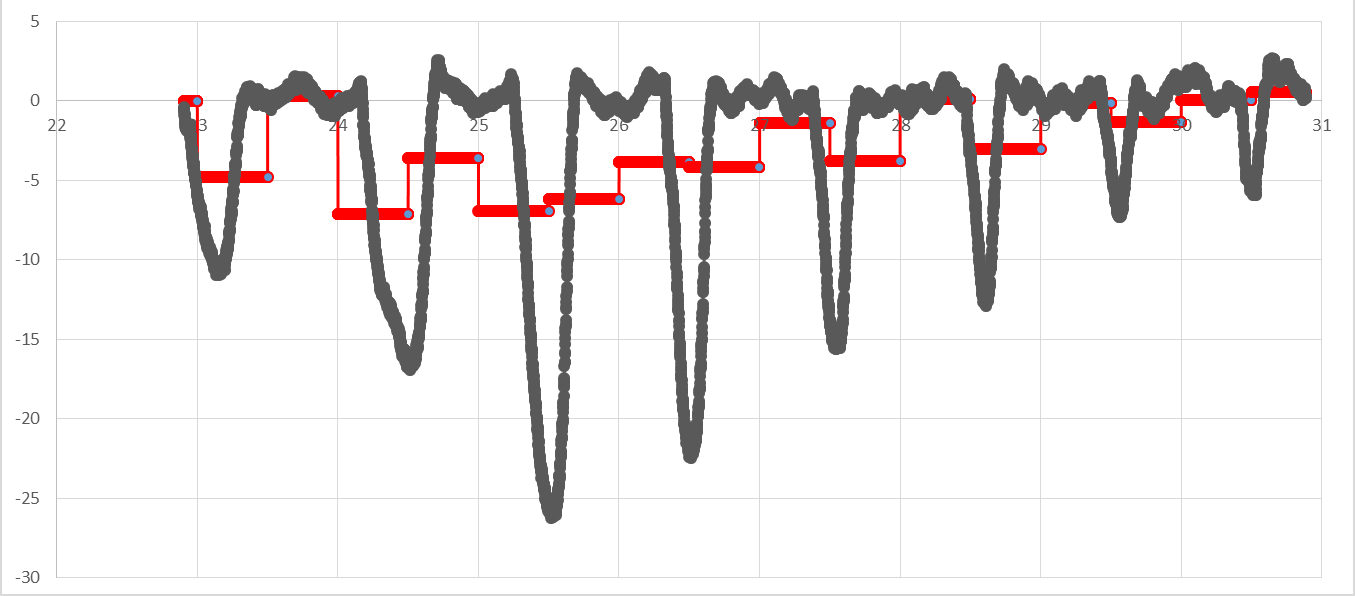
\includegraphics[scale=0.4]{images/sax-p/paa}
    \caption{Piecewise aggregate approximation of a cyclic time series}
  \label{fig:paa}
  \end{figure}

The main objective of PAA was to reduce the length of the time series. However, 
as it computes the segments means, it also allows us to compare two time series C and Q from 
the properties of their 
segments (Equation \ref{equ:paa} ).


\cite{lin2003symbolic} were based on the PAA method to provide a symbolic representation of time
series called Symbolic Aggregate Approximation (SAX). The objective of SAX is to assign a letter to
each segment. To do this, the domain of the values of the time series is divided into intervals
so that every point of the temporal series has approximately the same probability to belong to an 
interval and a letter is associated with each of these intervals.  Then each segment of the time
series is associated with the letter of the interval  to which belongs its average (Fig. \ref{fig:sax}).

 \begin{figure}[h]
  \centering
   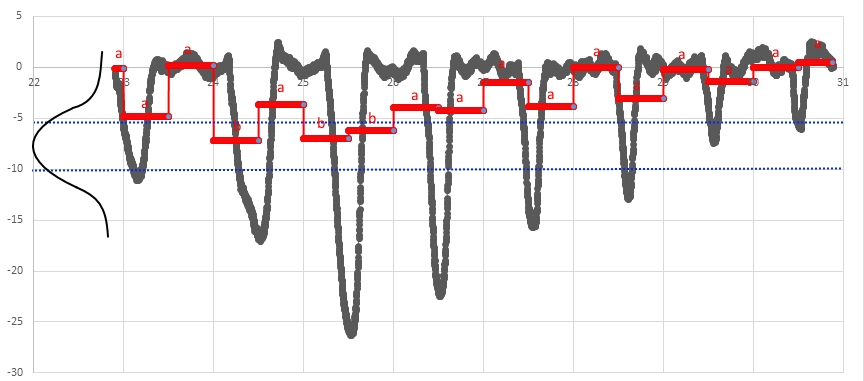
\includegraphics[scale=0.6]{images/sax-p/sax2}
    \caption{Symbolic Aggregate approXimation of a cyclic time series}
  \label{fig:sax}
  \end{figure}
	

With SAX, the distance $MINDIST$ between two strings $\hat{Q}$ and $\hat{C}$ of length $N$ is calculated from the
distance between the borders of the intervals represented by each character in the string 
(Equation \ref{equ:sax}).


\begin{equation}
MINDIST(\hat{Q},\hat{C})=\sqrt{\frac{n}{N}\sum_{i=1}^{N}(dist(\hat{q}_{i},\hat{c}_{i}))^{2}}
\label{equ:sax}
\end{equation}


$\hat{q}_{i}\:et\:\hat{c}_{i}$ are characters and $ dist() $ is the distance between the borders of 
the intervals which represent these characters  \cite{lin2003symbolic}. However, two segments with very 
different shapes can have the same average and be represented by the same letter: the mean is not 
enough to define a segment. In order to solve this problem, \cite{Lkhagva2006} proposed the ESAX 
model that considers three properties for each segment: its mean, its minimum and maximum (Fig. \ref{fig:esax}).

 \begin{figure}[h]
  \centering
   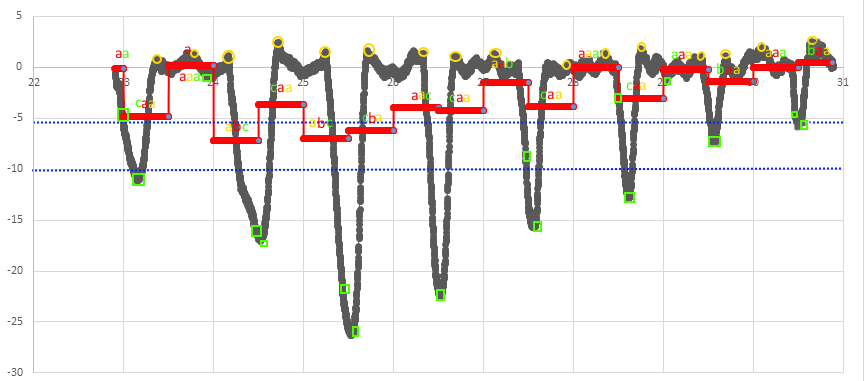
\includegraphics[scale=0.6]{images/sax-p/Esax}
    \caption{Extended Symbolic Aggregate approXimation of a cyclic time series}
  \label{fig:esax}
  \end{figure}

Thereafter, \cite{sun2014improvement} proposed the SAX-TD model that takes into account 
 two properties for each segment: its mean and trend. They then adjust the distance used by the SAX 
 method for it to take into account the trend (Fig. \ref{fig:saxtd}).

 \begin{figure}[h]
  \centering
   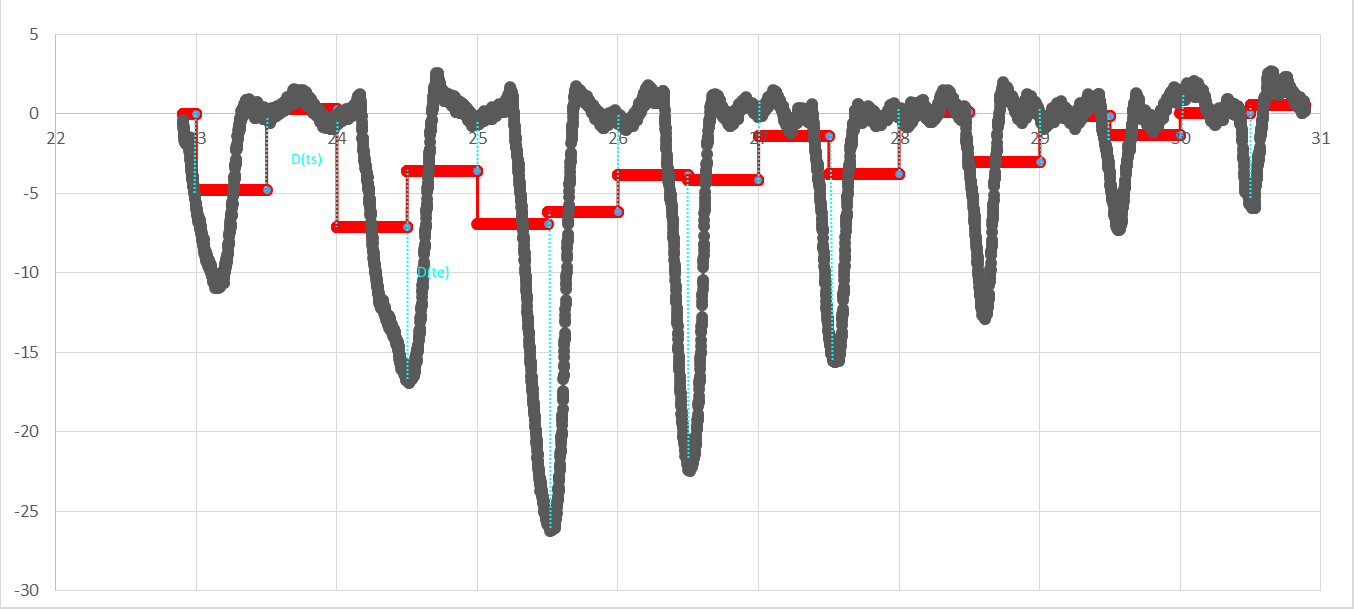
\includegraphics[scale=0.4]{images/sax-p/Sax-td}
    \caption{Trend Symbolic Aggregate approXimation of a cyclic time series}
  \label{fig:saxtd}
  \end{figure}
	
	 \begin{figure}[h]
  \centering
   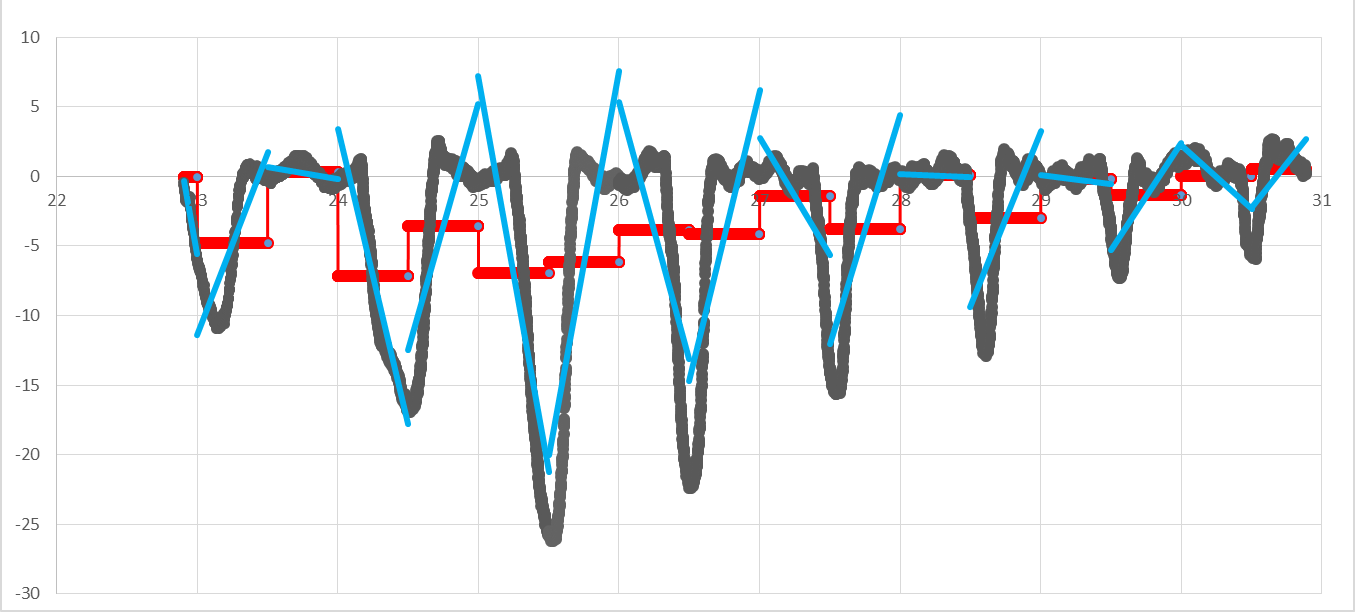
\includegraphics[scale=0.4]{images/sax-p/unD_sax}
    \caption{Properties of a cycle}
  \label{fig:1dsax}
  \end{figure}

Both methods provide better results than the SAX method \cite{sun2014improvement}. However, they have the
disadvantage of increasing the number of symbols required to represent the time series. Indeed, 
the method ESAX triple the size of the representation of a time series provided by the SAX method, 
while the SAX-TD method the double. In addition,  the previous four methods have two major drawbacks: 
they consider fixed-size segments, while the cycles are variable-sized segments, and they do not take into account the characteristic properties of cycles such as 
the duration and the surface under a cycle. Our goal is to provide a symbolic representation that 
takes into account several properties for each cycle, but without increasing the number of symbols 
used for the representation.


 The symbolic representations obtained have another advantage;
they allow to use a large number algorithms available
for sequence analysis like novelty detection (finding
unusual shapes or sub-sequences), motif discovery (finding
repeated shapes or sub-sequences) \cite{Begum2014}, clustering, classification,
indexing and also some interesting algorithms for
text processing or the bio-informatics community \cite{Aach2001, Papapetrou2011, Dietterich2002}. 

\section{SAX-P}

A prerequisite to be able to build a symbolic representation based on the cycles of the cyclic time series is to be able to segment the cyclic time series into consecutive cycles.

\subsection{Segmentation of cyclic time series}
The principle used to segment cyclic time series is as follows: A cycle contains all the data points between the beginning of two consecutive peaks. To locate the peaks, we set a threshold (Fig. \ref{fig:seuil}). The threshold considered can be the first or the second quartile of the time series data point.

	 \begin{figure}[h]
  \centering
   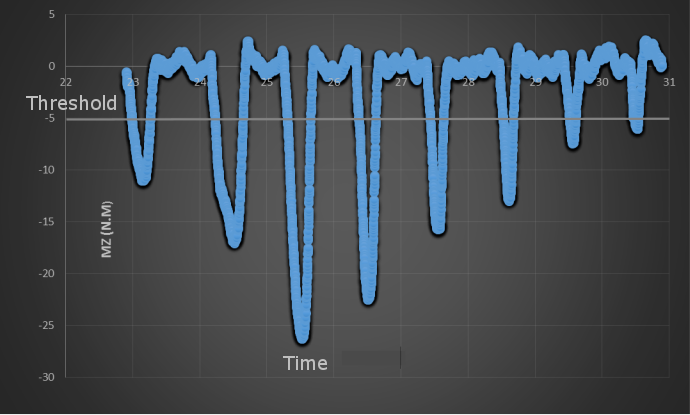
\includegraphics[scale=0.4]{images/sax-p/sax-p_deplacement_seuil}
    \caption{Threshold for the segmentation of cyclic time series}
  \label{fig:seuil}
  \end{figure}

If the current value of the time series is below this threshold, then it is a peak. It is then necessary to turn back to find the moment of the beginning of the peak. The figure (Fig. \ref{fig:segmentation}) presents the results obtained after segmentation of a cyclic time series.

	 \begin{figure}[h]
  \centering
   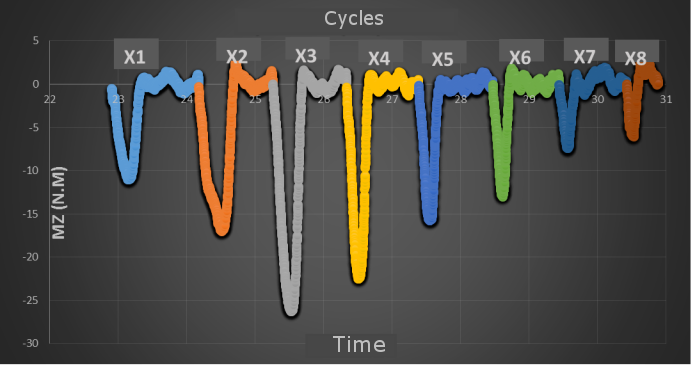
\includegraphics[scale=0.4]{images/sax-p/sax-p_deplacement32_thesee}
    \caption{Segmentation}
  \label{fig:segmentation}
  \end{figure}
	
\subsection{From cycles to letters}
The method SAX-P is based on SAX and works as follows:  
\begin{enumerate}
\item A cyclic time series is split in successive segments using a threshold
for identifying the beginning and the end of cycles, which have variable
durations;	
\item Several parameters (properties) are computed on each segment: cycle
time, push time, mean, median, standard deviation, minimum and maximum
values, and the area under the time series curve. As all these parameters
have different units, they must be normalized (i.e. centered and reduced) (Fig. \ref{fig:property} );

	 \begin{figure}[h]
  \centering
   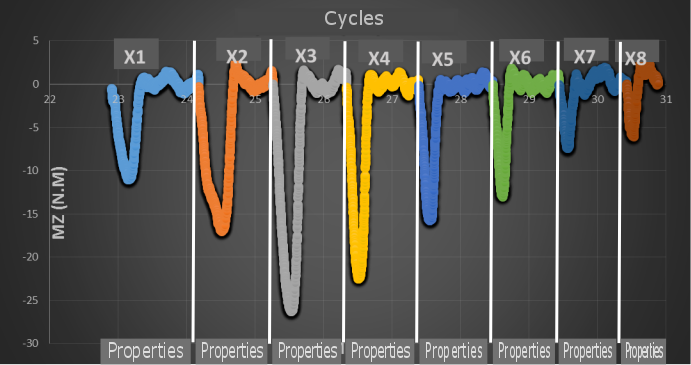
\includegraphics[scale=0.4]{images/sax-p/sax-p_deplacement_property}
    \caption{Some properties are computed on each cycle}
  \label{fig:property}
  \end{figure}
	
 
\item Segments are then gathered in clusters using a classification algorithm
\cite{Esling2012} and each cluster is named by a capital letter (Fig. \ref{fig:classification}); 

	 \begin{figure}[h]
  \centering
   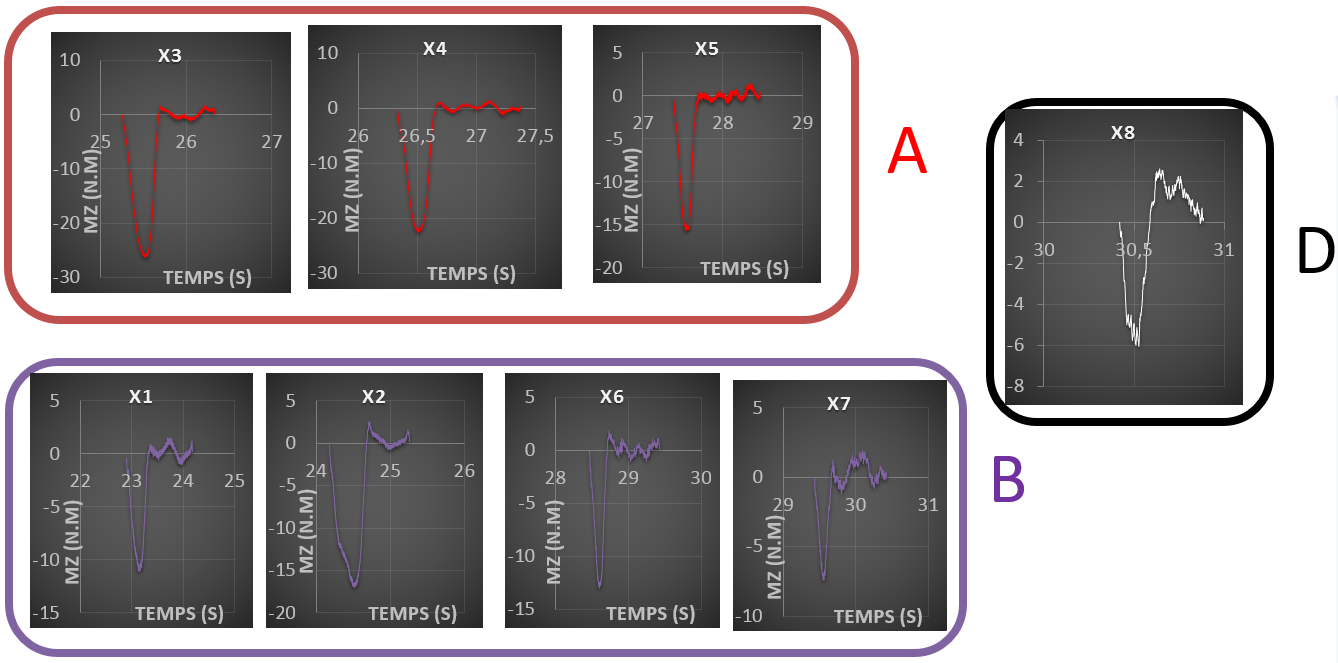
\includegraphics[scale=0.4]{images/sax-p/regroupement}
    \caption{Classification of cycles based on properties}
  \label{fig:classification}
  \end{figure}
	
	
\item Each segment is replaced by the letter of the cluster to which it
belongs, so that the initial cyclic time series is then represented
by a string of characters (Fig. \ref{fig:symbolic}); 

	 \begin{figure}[h]
  \centering
   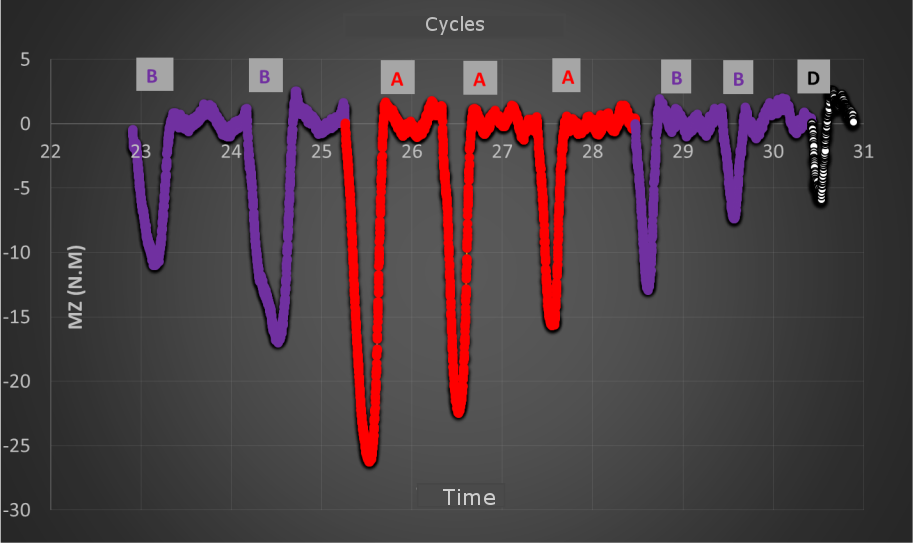
\includegraphics[scale=0.4]{images/sax-p/representionSymbolique2_t}
    \caption{Symbolic representation of cyclic time series}
  \label{fig:symbolic}
  \end{figure}
	
 \end{enumerate}

The distance between two strings, which may have different numbers
of characters, is computed using Dynamic Time Warping \cite{Petitjean2014} which is known as the
best distance measure for several domains \cite{Ding2008}. The distance between two characters is
the euclidean distance between the centers of the classes represented by those characters.

Unlike SAX, ESAX and SAX-TD methods that require  to fix the length of segments to consider when 
building the symbolic representation of a time series, SAX-P considers the cycles which
constitute basic unit of analysis of time series recorded during cyclic movements and also 
allows taking into account several characteristic features for each cycle. Figure \ref{fig:symbolic}
presents the symbolic representations obtained with the SAX method (in small letters) and SAX-P (in
capital letters). It illustrates that SAX-P unlike SAX considers cycles of the time series during
the construction of the symbolic representation.

%\begin{figure}[ht]
%\vskip 0.2in
%\begin{center}
%\centerline{\includegraphics[width=\columnwidth]{methode.png}}
%\caption{A cyclic time series is segmented in 5 propulsion cycles  
%(X1, X2, X3, X4, X5). For each cycle, a set of properties was 
%calculated and cycles with similar properties are gathered in 
%the same class (A or B). The original time series is thus transformed 
%into a string (here: AAABB).}
%\label{fig:methode}
%\end{center}
%\vskip -0.2in
%\end{figure} 

%\begin{figure}[ht]
%\vskip 0.2in
%\begin{center}
%\centerline{\includegraphics[width=\columnwidth]{representationS2.png}}
%\caption{Example of cyclic time series: propulsive moment applied by
% the subject S1  to the rear wheel of a Manual Wheelchair for a rectilinear
%  movement. Vertical bars delimit the propulsion cycles (segments) 
%  identified during this run, and the capital letter above each 
%  cycle indicates the cluster to which it belongs. Applying SAX to the propulsive moment divide
%  the time series into 10 segments of equal size (lowercase letter) regardless of propulsion cycles.
%  The area under the cycle, the cycle time and the pushed time are not taken into account by SAX.}
%\label{fig:moment}
%\end{center}
%\vskip -0.2in
%\end{figure} 

\section{Application to manual wheelchair locomotion}
This method has been applied to the axial moment (Mz) measured by both right and left rear wheels of
an instrumented Manual WheelChair (MWC) during five there and back 10-m linear displacements between
two cones performed by three handicapped subjects. We group propulsion cycles into 5 clusters  (Table
\ref{tab:centroide}) and we obtained a symbolic representation for Mz (Table
\ref{tab:symbole}).




\begin{table}
\center
\begin{tabular}{|c|c|c|c|c|c|}
\hline 
Cluster & A & B & C & D & E\tabularnewline
\hline 
\hline 
Nb of cycles & 18 & 36 & 59 & 18 & 104\tabularnewline
\hline 
\textbf{Cycle time (s)} & 1.2 & 1.0 & 1.0 & 1.7 & 0.8\tabularnewline
\hline 
\textbf{Push time (s)} & 0.6 & 0.3 & 0.4 & 1.0 & 0.3\tabularnewline
\hline 
Mz Min (Nm) & -22.3 & -17.4 & -11.4 & -8.7 & -6.4\tabularnewline
\hline 
Mz Max (Nm) & 0.1 & 0.1 & 0.1 & 0.7 & 0.1\tabularnewline
\hline 
Mean (Nm) & 13.6 & -8.1 & -6.2 & -3.0 & -3.3\tabularnewline
\hline 
Median (Nm) & -16.1 & -10.8 & -7.4 & -4.2 & -3.9\tabularnewline
\hline 
IRQ (Nm) & 12.4 & 10.7 & 6.0 & 4.3 & 3.1\tabularnewline
\hline 
SD (Nm) & 7.1 & 5.6 & 3.4 & 2.6 & 1.8\tabularnewline
\hline 
\textbf{Area (Nm.s)} & -7.1 & -2.3 & -2.2 & -1.8 & -1.0\tabularnewline
\hline 
\end{tabular}\protect\caption{Average vectors of the properties of classes (A, B, C, D, E) used
for the symbolic representation of the axial moment (Mz) SAX-P takes into account 
the surface under the push, the time-push and
the time-cycle.}
\label{tab:centroide}
\end{table}





\begin{center}

\begin{table}
\center
\begin{tabular}{|c|c|c|c|c|c|c|}
\hline 
Subject & \multicolumn{2}{c|}{S1} & \multicolumn{2}{c|}{S2} & \multicolumn{2}{c|}{S3}\tabularnewline
\hline 
\hline 
Push & Right & Left & Right & Left & Right & Left\tabularnewline
\hline 
1 & C & A & C & D & E & D\tabularnewline
\hline 
2 & B & B & E & E & D & E\tabularnewline
\hline 
3 & B & B & C & E & C & E\tabularnewline
\hline 
4 & B & B & C & E & E & E\tabularnewline
\hline 
5 & B & B & C & D & E & E\tabularnewline
\hline 
6 & C & B & E & C &  & D\tabularnewline
\hline 
7 & B & C & E & E &  & E\tabularnewline
\hline 
8 & E &  & E & E &  & \tabularnewline
\hline 
9 &  &  & C & C &  & \tabularnewline
\hline 
10 &  &  & E & E &  & \tabularnewline
\hline 
11 &  &  & C & E &  & \tabularnewline
\hline 
12 &  &  & C & E &  & \tabularnewline
\hline 
13 &  &  &  & E &  & \tabularnewline
\hline 
DTW & \multicolumn{2}{c|}{268} & \multicolumn{2}{c|}{354} & \multicolumn{2}{c|}{44}\tabularnewline
\hline 
\end{tabular}

\protect\caption{Strings of characters obtained with SAX-P method on times series of
axial moments applied by the three subjects on right and left rear
wheels of an instrumented MWC during their second 10-m run.}
\label{tab:symbole}

\end{table}

\end{center}





An important task of analyzing manual wheelchair locomotion 
 is the comparison of its rolling movement. Experts from the fields seek to 
 compare two movements simultaneously taking into account 
 several criteria or properties. Applying SAX-P method to the time series 
 of axial moments exerted
by a wheelchair user on the right and left wheels greatly
facilitates the comparison, the analysis and the interpretation of these time series: 
\begin{itemize}
\item At first sight (Table 2), it immediately appears that during their
second 10-m run the three subjects analyzed here did not exert the
same number of pushes for moving a MWC on the same distance (S1:
7-8; S2: 12-13; S3: 5-7); 
\item It is also obvious that each subject did not exert the same number
of pushes on both rear wheels. Moreover, although right and left pushes
exerted by one subject globally belong to the same clusters, the total
distance between all these pushes can be more (S2: 354) or less (S3:
44) high. Both these observations clearly demonstrate that the three
subjects did not propel their MWC symmetrically during this particular
exercise. The first results of the evaluation of SAX-P on a classification task are presented on
the web page \cite{Validation}
\end{itemize}


\section{Conclusion}
In this ongoing work, we proposed a method of symbolic representation of cyclic time series called SAX-P.
This method is used to represent a cyclic time series as a string, each character representing a
class of the cycles of the considered time series. The character strings
obtained were then compared using the Dynamic Time Warping distance.
 The SAX-P model has been applied to propulsive moments measured during the movements in a straight
 line by three subjects in MWC. The preliminary results obtained have particularly showed that these
 subjects had different modes of propulsion and propulsion cycles of the same subject were not 
 symmetrical. Ongoing research is devoted on applying this new symbolic representation to a 
 supervised classification of cyclic time-series in bio-mechanics.